%\newpage
\section{ENGINEERING REQUIREMENTS}

\subsection{System Overview} 
The Backyard Splash Pad is comprised of four main components: a device controller, a user interface, a mechanical system, and an object-tracking system. 
The device controller receives input from the user interface and uses it to control the mechanical system.
The user interface presents information about the system to the user and accepts input from the user.
The mechanical system controls the flow of water. 
The object-tracking system detects objects near the Splash Pad and reports information to the controller. 
See Figure \ref{fig:functional_diagram}.

\subsubsection{Functional Diagram}

\begin{figure}[h]
\centering
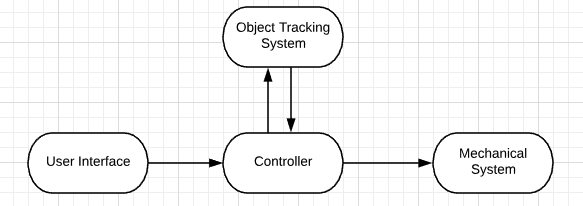
\includegraphics[width=0.9\textwidth]{Functional_Diagram.png}
\caption{\label{fig:functional_diagram}Functional Diagram.}
\end{figure}

\subsection{Functional Requirements}

\subsubsection{Controller}
%The controller is the part of the system that controls the physical outputs. 

\paragraph{Stream Control}
The controller shall be able to turn on and off each water stream individually.

\paragraph{Light Control}
The controller shall be able to turn on and off each light individually.

\paragraph{Color Control}
The controller shall be able to change the color of each light individually.

\paragraph{Responsive to Object Tracking System} 
The controller shall be able to turn on a specified nozzle as directed by the Object Tracking System.

\paragraph{Programmed Display}
The controller shall have at least one pre-programmed fountain routine containing light changes and water streams turning on and off.

\subsubsection{User Interface}
%The user interface is the part of the system that accepts input from the user and translates it into commands that the controller can execute. 

\paragraph{User Nozzle Control}
The user interface shall allow the user to select what nozzle(s) are turned on.

\paragraph{User Color Control}
The user interface shall allow the user to select what color the LEDs are.

\paragraph{User Object Tracking Control}
The user interface shall allow the user to enable or disable the object tracking system.

\subsubsection{Mechanical System}
%The mechanical system is the physical aspect of the system. The mechanical system produces all of the functional output of the system. 

\paragraph{Water Flow}
The mechanical system shall be able to create seven water streams that rise at least 6.0 ft vertically above the nozzle.

\paragraph{Water Protection}
%The mechanical system shall conform to the IP65 standard.   
The mechanical system shall be sprayproof. %Test in MIL-STD-108 in accordance with test described in 4.9

\paragraph{Dust Protection}
The mechanical system shall be dust-tight. %Test in MIL-STD-810 in accordance with section 510.5. 

%MIL-STD-108 has ingress protection information.
%MIL-STD-810 has environmental protection information.

\paragraph{Play Surface}
The mechanical system shall provide a play surface capable of supporting at least 500.0 pounds.

\paragraph{Operation Time}
The mechanical system shall be able to operate for 10,000 hours. 

\paragraph{Safety}
Electrical components in the mechanical system shall conform to section B.4 in MIL-STD-1310H. 

%MIL-STD

%TODO: NEED TO WORK ON THIS
%Ask Dr. Cripps how to get access to standards. 
%Answer: Use every-spec



\subsubsection{Object Tracking System}
%The Object Tracking System is the part of the system that senses objects in the area surrounding the splash pad, and sends commands to the controller based on the position of objects detected.

\paragraph{Minimum Object Size}
The Object Tracking System shall be able to detect any object larger than a sphere with a 9.4 in. diameter that is within 2.0 ft of any nozzle.

\paragraph{Lighting Levels}
The Object Tracking System shall be able to function when the brightness level around the splash pad is at least 2000 lux.

\paragraph{Automatic Calibration}
The Object Tracking System may be able to automatically adjust to differences in its position relative to the splash pad if its position changes. 

\subsection{Support Requirements}

\subsubsection{Device Controller}
%TODO:  Come up with support requirements for this.
The Device Controller shall have labeled buttons.

%\paragraph{User Interface}
%The User Interface shall require an android phone for advanced features. 
%TODO:  Come up with support requirements for this.
%\paragraph{Interface Platform}  %I got rid of this because isn't the controller essentailly the interface platform?


\subsubsection{Mechanical System}

\paragraph{Power Consumption}
The system shall operate on 1000.0 Watts or less.

\paragraph{Power Supply}
The system shall be powered by a standard 120 V electrical outlet. 
%Needs to be safe.

\paragraph{Size}
The system shall fit within a cube that is 10 ft on an edge.
%TODO: Mechanical constraints are light. 

\paragraph{Water Conservation}
%TODO: James, put a percent sign in here...
The system shall reuse at least 50\% of the water. %I only put 50 due to evaporation and what gets soaked into clothes.

%\paragraph{Water Pressure}
%There shall be a way to regulate the water pressure inside of the system.

\paragraph{Nozzles}
The Nozzles shall create laminar flowing streams of water.

%\subsubsection{Object Tracking System}

%\paragraph{Size}
%The object tracking system shall fit within a cube that is 6 inches on a side.

%\paragraph{Container}
%The object tracking system shall have an enclosure.  

%\paragraph{Mounting}
%The object tracking system case shall have a mounting interface. 


%%%%%%%%%%%%%%%%%%%%%%%%%%%%%%%%%%%%%%%%%%%%%%
%specs to add
%%%%%%%%%%%%%%%%%%%%%%%%%%%%%%%%%%%%%%%%%%%%%%
%Construction Quality
%Safety Standards
%
%
%%%%%%%%%%%%%%%%%%%%%%%%%%%%%%%%%%%%%%%%%%%%%%
%\begin{quote}
	%\input{CourseInstructorMounting}
%\end{quote}
%
%Now is good time to discuss the difference between design constraints and requirements.  Why don't we treat the rail mounting constraint as a requirement?  We could and often we would by simply specifying an exact mounting structure for the power amplifier with no explanation of why it has to be the size and shape that it must be.  However, the rail mounting system is an external standard that we must follow and my experience tells me that informing the designer of the reason for this constraint keeps the designer happier.  And happier designers mean happier spec writers!
%\bigskip
%
%At this point we can simply state the fundamental constraint and leave the actual mounting envelope sizes to another place in the document (probably the Interface section) or we can state the complete requirement here.  I choose to put it here and back reference it in the requirements simply because it is a constraint and splitting the needed data into two places could lead to interpretation errors.  The rail mounting constraint follows.
%\bigskip
	%
%\end{slshape}
%
%\subsubsection{Rail Mounting Constraint}
%
%
%\paragraph{} 
%
%The controls lab power amplifier module shall be packaged in a structure that mounts to the 1 inch t-slot railing used in the lab via two $1/4$ inch holes in the bottom of the structure that are separated by no more than two inches.
%
%\paragraph{} 
%
%The module package dimension along the rail shall be no more six inches.
%
%\begin{slshape}
%\color{blue}
%
%We can now look for other constraints in the stakeholders' user stories.  The last course instructor user story uses indefinite words such as 'need', `can', and `recommended'.  These words imply latitude in implementation and as such will be expanded in the appropriate requirements section.
%\bigskip
%
%The lab instructor user stories yield needs no specific constraints.  Remember even a specific requirement is not a constraint if no specific method is expressed.
%\bigskip
%
%The lab student user stories also have needs but without expressing specific methods.  No constraints here.
%\bigskip
%
%The USU ECE Department user stories have flirtations with constraints but never quite get there with phases such as `must be a simple' and 'should cost less'.  While the Department may be sincere about these requirements they are not constraining the designer to a specific method to achieve them (they aren't even really requiring them).
%\bigskip
%
%\end{slshape}
%
%\subsection{Functional Requirements}
%
%\begin{slshape} \color{blue}
	%A quantitative statement of how the item does what is
	%does. For a thruster it would be thrust, specifc impulse and stability. For a power supply
	%it would be current, voltage, and efficiency. Times like rise times, fall times, and
	%transients are defned here. Leakage (uid or current) is usually defined here.
	%Compatibility with fluids is often defined here. It is a good idea to start with a previous
	%spec for a similar item to get some ideas for all that may need to be in this section.
	%Curves, truth tables, and functions are often better than words for these requirements.	
%\end{slshape}
%
%\subsubsection{Amplifier Functional Characteristics}
%
%\paragraph{Voltage Gain Requirement}\label{gainSpec}
%
%The controls lab power amplifier shall have the following steady state transfer function (voltage gain):
%\bigskip
%
%\begin{math}
	%\dfrac{V_{out}}{V_{in}} = 1.0 \pm 1\%
%\end{math}
%
%\paragraph{Output Current Requirements}
%
%The controls lab power amp shall have a maximum steady state output current of no less than 8 amps.
%
%\paragraph{Bandwidth}
%
%The controls lab power amplifier shall have a half power bandwidth of no less than 100 Hz.
%
%
%
%\subsection{Non-Functional Requirements}
%
%\begin{slshape} \color{blue}
%
%What follows is a really long (and yet strangely incomplete) list of potential non-functional requirements.  You will likely have noticed that the functional requirements for the controls lab power amplifier is a pretty short list.  Simple signals in and out and a frequency response requirement.  We should be able to stop this madness now and build the thing.  Sadly, we can't stop yet.
%\bigskip
%
%The device functions described in the section above don't and can't stand alone.  These functions require a lot of support from the environment.  To use a common example, the functions of a cell phone are simply dreams without the battery,  The functions of that same phone are useable only because of an effectively designed package.  Your cell phone is useful over a range of temperatures (a much smaller range than you are likely aware of (\href{https://support.apple.com/en-us/HT201678}{iPhone Temperature Ranges})) because the designers made it useful over the range of temperatures that were specified.  In short, function is meaningless without a non-functional framework or, in other words, a functional support framework.
%\bigskip
%
%Our example is no different.  The amplifier must be supplied with power.  It must be able to operate over a range of temperatures and dissipate heat so as to keep the amplifying element safe.  It must be packaged to make it possible for us to actually use it.  We specify those requirements in this section and include the list of a bunch of others that may or may not apply to our specific project.
%\bigskip
%
%Returning to the user stories we look for the requirements that the users have provided that can be classified as non-functional requirements.  The first one we encounter deals with the electrical wiring and it seems reasonable then to group electrical support (non-functional) issues into their own section.  The course instructor requires:
%\bigskip
%
%\WiringErrors
%\bigskip
%
%Looking for more electrical requirements we find:
%\bigskip
%
%\OverCurrent
%\bigskip
%
%and the lab instructor suggests:
%\bigskip
%
%\BananaJacks
%\bigskip
%
%The lab instructor requires:
%\bigskip
%
%\UserWiringInterface
%
%
  %
%
%Lets' divide this section into the following subsections:
%
%\begin{itemize}
	%\item Electrical Requirements
	%\begin{itemize}
		%\item Power Protection Requirements
		%\item Connector Requirements
	%\end{itemize}
	%\item{Environmental Requirements}
	%\begin{itemize}
		%\item Operating Temperatures
		%\item Power Dissipation
	%\end{itemize}
	%\item Physical Characteristics
	%\begin{itemize}
		%\item Packaging
		%\begin{itemize}
			%\item Package Envelope
			%\item Rail Mount
		%\end{itemize}
	%\end{itemize}
%\end{itemize}
%
%Starting with the electrical requirements we continue our example.
%\end{slshape}
%
%\subsubsection{Electrical Requirements}
%
%\begin{slshape} \color{blue}
%
%\end{slshape}
%
%\paragraph{Power Protection Requirements} 
%
%\begin{slshape} \color{blue}
%
%\end{slshape}
%
%\paragraph{Connector Requirements}
%
%\subsubsection{Environmental Requirements}
%
%\begin{slshape} \color{blue}
%{\underline{Environments}}
	%
	%\bigskip
%
	%This section is for anything and everything that is external 
	%to the item that it must withstand. Customers may impose these with an 
	%Environmental Requirements Document. Margins should be added beyond 
	%hard environmental limits that would damage the item. NOTE: MOST OF THIS 
	%IS THE SAME FOR ALL SUBSYSTEMS AND WILL THEREFORE BE WRITTEN INTO THE 
	%SYSTEMS SPEC.
	%
	%\bigskip
%
	%{\underline{Natural Environments}}
	%
	%\bigskip
%
	%Anything that is relevant to the item that can occur in the 
	%natural world, either prior to use or during use. Some words like 
	%"The item shall meet the requirements of this specification 
	%during and after exposure to any combination of any of the following 
	%natural environments. The item may be packaged to precluded exposure to 
	%any environments that would control the design." Typical environments 
	%include (but are not limited to):
	%
	%\bigskip
%
	%External Pressure, remember barometric and transportation in 
	%unpressurized aircraft. Also rate of pressure change.
	%
	%\bigskip
%
	%Temperature including both operating and non-operating. Some 
	%special temperatures may include freezing points of consumables like 
	%fuels.
	%
	%\bigskip
%
	%Salt spray or other corrosives, lightning, and magnetic fields.
	%
	%\bigskip
%
	%{\underline{Induced Environments}}
	%
	%\bigskip
%
	%Anything that is relevant to the item that is caused by 
	%human-made objects, either prior to use or during use. Some words like 
	%\textsl{"\,The item shall meet the requirements of this specification 
	%during and after exposure to any logical combination of the following 
	%natural environments." } Typical environments include (but not limited 
	%to):
	%
	%\bigskip
%
	%Mechanical shock, including transportation and use. Amplitude and 
	%number of shocks can be defined in either the time domain or frequency 
	%domain.
	%
	%\bigskip
%
%
	%Vibration, including transportation and use. Amplitude as a 
	%function of frequency is the usual format. Duration is a key part of 
	%this requirement.
	%
	%\bigskip
%
	%Acoustic input
	%
	%\bigskip
%
	%Load factors and acceleration
	%
	%\bigskip
%
	%Space Environment including Radiation, Atomic Oxygen. Radiation is 
	%a specialty area that includes cosmic radiation, charged particles in 
	%the solar wind and Van Allen radiation in some orbits. Atomic oxygen is 
	%of concern for polymers and nonmetallic materials exposed on the front 
	%of the spacecraft (with reference to the velocity vector) in orbits 
	%under 500 km altitude.
	%
	%\bigskip
%
	%Spacecraft develop charges when moving through the earth's 
	%magnetic field in the continuous presence of charged particles. 
	%Increased solar wind can alter the magnitude of the charge. Design 
	%features may be needed to diminish charge separation within a 
	%spacecraft, make electronics less vulnerable to accumulated charge, and 
	%in the case of rendezvous and docking allow for harmless dissipation of 
	%accumulated charges between spacecraft.
	%
	%\bigskip
%
	%External Pressure, remember barometric and transportation in 
	%unpressurized aircraft. Also rate of pressure change.
	%
	%\bigskip
%
	%Temperature during operation. Also thermal cycling and 
	%thermal/vacuum. 
	%
	%\bigskip
%
%
	%Cleanliness: Cleanliness is, of course, next to Godliness, and that is 
	%even more true that you realize for spaceflight hardware. This section 
	%usually controls particulate and fiber cleanliness with tables of 
	%allowable count per range of particle size. Surface cleanliness is also 
	%controlled. The use and certification of cleanrooms is controlled in 
	%this section. Special issues such as propellant contacting surfaces, 
	%flushing fluid components, and electronic cleanliness are controlled 
	%here. NOTE: MOST OF THIS IS THE SAME FOR ALL SUBSYSTEMS AND WILL 
	%THEREFORE BE WRITTEN INTO THE SYSTEMS SPEC.
	%
	%\bigskip
%
	%Electromagnetic interference (EMI):  The unit shall met the EMI 
	%requirements for class xxx equipment as specified in 
	%MIL-STD-461, except for yyy limits shall be modified as shown 
	%in Figure zzz.  This is typical language, and MIL-STD-461 
	%is still commonly used. Emissions, refer to EMI that originates in the 
	%unit that can negatively affect other things. Susceptibility refers to 
	%unexpected negative effects on the unit that are caused by emissions 
	%from some other source. Self-susceptibility is a special case when 
	%electrical noise created by the unit triggers and unexpected effect 
	%within the unit. EMI can be "conducted" along power or 
	%signal wires or "radiated." The MIL-STD-461 limits have coded names 
	%like:
	%
	%\bigskip
%
	%CS01 = conducted susceptibility in the first frequency range, RE02 = 
	%radiated emissions in the second frequency range.
	%
	%\bigskip
%
	%Magnetic fields are another category controlled by the MIL-STD. Testing 
	%methods are usually defined by an associated methods document, 
	%MIL-STD-462. Other parts or sub-paragraphs in this section deal with 
	%electrical bonding (specified minimum resistance) between different 
	%subassemblies, EMI gasket and screen materials, grounding, lightning 
	%transients, and shielding.
%\end{slshape}
%
%\subsubsection{Physical Characteristics}
%
%\begin{slshape} \color{blue}
%{\underline{Physical Characteristics}}
	%
	%\bigskip
	%This is the place for the envelope drawing that shows size 
	%and general configuration. Sensitive areas, keep-out zones, and dynamic 
	%envelopes should be defined here. The mass, mass moment of inertia, 
	%center of mass, and natural frequency requirements can be defined here. 
	%Any unusual orientation requirements (e.g. "\,this side up") can be 
	%defined here. Location requirements for electrical connectors or 
	%tube-fitting interfaces should be defined. Visual indicators or 
	%inspection zones or tool access zones should be identified.
	%
	%\bigskip
%\end{slshape}		